\documentclass[11pt]{article}

\usepackage[letterpaper, margin=1in]{geometry}

\usepackage[spanish]{babel}
\usepackage[utf8]{inputenc}
\usepackage{multirow}
\usepackage{tabularx}
\usepackage{longtable}



%Figuras
\usepackage{graphicx, subfigure}
\usepackage[]{tikz}
\usepackage{pbox}

%Matemática
\usepackage{amsmath}
\usepackage{amssymb}

%Símbolos mate extra (alfabetos, etc.)
\usepackage{mathrsfs}


%Algoritmos
\usepackage{float}
\usepackage{algorithm}
\usepackage{algorithmicx}
\usepackage{algpseudocode}
\usepackage{listings}


\usepackage{color}
\usepackage{hyperref}

\usepackage{mdframed}
\usepackage{tcolorbox}
\usepackage{multicol}
\usepackage{booktabs}
\usepackage{tabulary}
\definecolor{darkblue}{rgb}{0 , 0.054 , 0.196}



\title{Reporte de Laboratorio 1\\Punteros y funciones en C++}
\author{Dunia Barahona - B40806}
%otro autor se pondría así \author{nombre1\\nombre2}
\begin{document}

\maketitle
\hrule
\hrule
\tableofcontents
\hspace{5mm}
\hrule
\hrule

\section{Código}
A continuación se mencionan las funciones del programa.
\begin{itemize}
	\item \texttt{cont}: obtiene el tamaño del código genético (ARN) ingresado desde la línea de comandos.
	
	\begin{figure}[H]
		\centering
		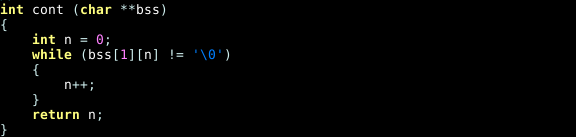
\includegraphics[scale=0.9]{cont.png}
		\caption{función \texttt{cont}}
		\label{fig:fcont}
	\end{figure}
	\newpage
	\item \texttt{amino}: determina cual aminoácido corresponde al codón de ARN ingresado según la tabla de conversión ARN a aminoácido.
	
	\begin{figure}[H]
		\centering
		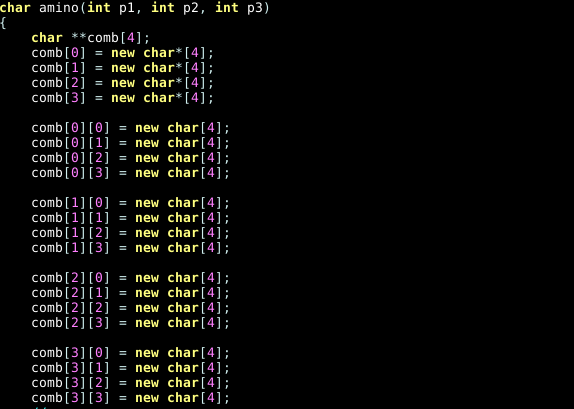
\includegraphics[scale=0.9]{amino_1.png}
		\caption{tabla de conversión ARN-aminoácido}
		\label{fig:fam1}
	\end{figure}
	
	\begin{figure}[H]
		\centering
		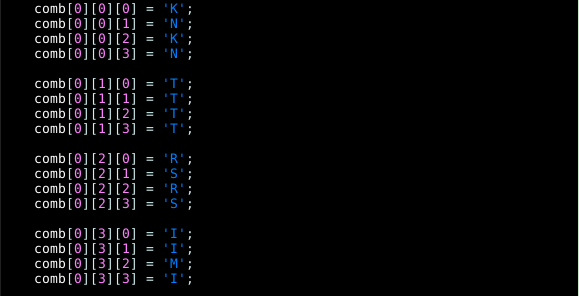
\includegraphics[scale=0.9]{amino_2.png}
		\caption{tabla de conversión ARN-aminoácido}
		\label{fig:fam2}
	\end{figure}
	
	\begin{figure}[H]
		\centering
		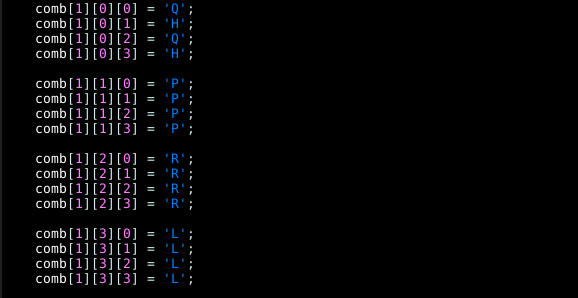
\includegraphics[scale=0.9]{amino_3.png}
		\caption{tabla de conversión ARN-aminoácido}
		\label{fig:fam3}
	\end{figure}
	
	\begin{figure}[H]
		\centering
		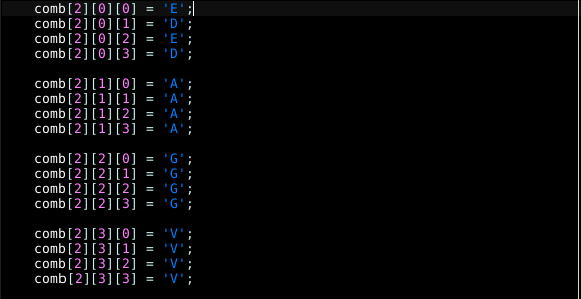
\includegraphics[scale=0.9]{amino_4.png}
		\caption{tabla de conversión ARN-aminoácido}
		\label{fig:fam4}
	\end{figure}
	
	\begin{figure}[H]
		\centering
		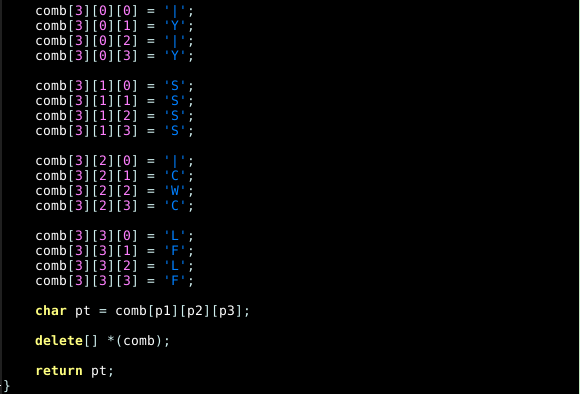
\includegraphics[scale=0.9]{amino_5.png}
		\caption{tabla de conversión ARN-aminoácido}
		\label{fig:fam5}
	\end{figure}
	\newpage
	\item \texttt{triplete}: traduce las bases del codón recibido según lo siguiente: A= 0, C= 1, G= 2, U= 3.
	
	\begin{figure}[H]
		\centering
		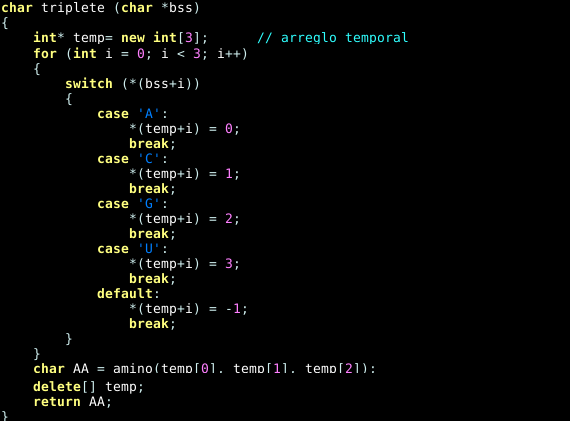
\includegraphics[scale=0.9]{triplete.png}
		\caption{función \texttt{triplete}}
		\label{fig:ftri}
	\end{figure}
	
	\item \texttt{insp}: verifica si el ARN ingresado cumple con las siguientes condiciones:
	\begin{enumerate}
		\item La cantidad de bases que lo componen es multiplo de 3.
		\item  Está compuesto únicamente por los caracteres que corresponden a bases nitrogenadas (A, C, G, U).
	\end{enumerate}
	
	\begin{figure}[H]
		\centering
		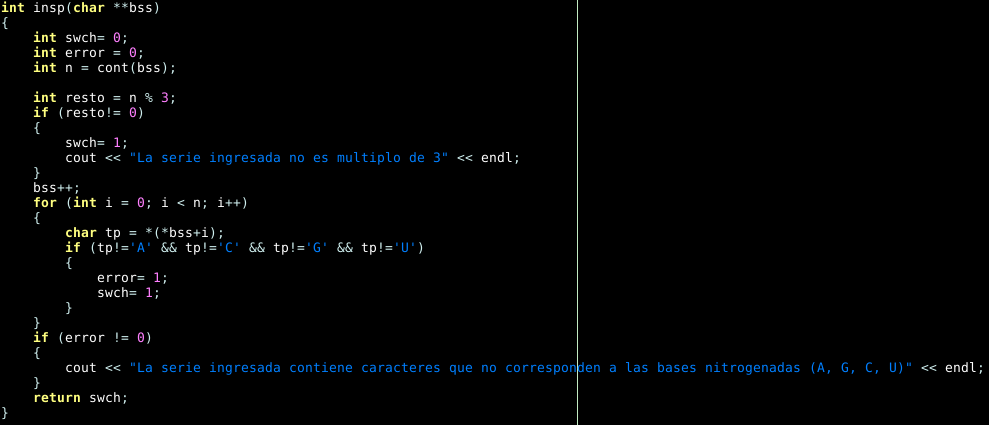
\includegraphics[scale=0.6]{insp.png}
		\caption{función \texttt{insp}}
		\label{fig:finsp}
	\end{figure}
	
	\item \texttt{traducirARNaAA}: tiene como parámetro un puntero de char \texttt{char** arn} el cual contiene la dirección de memoria del ARN ingresado desde la línea de comandos y retorna un nuevo arreglo de char con los animoácidos resultantes.
	
	\begin{figure}[H]
		\centering
		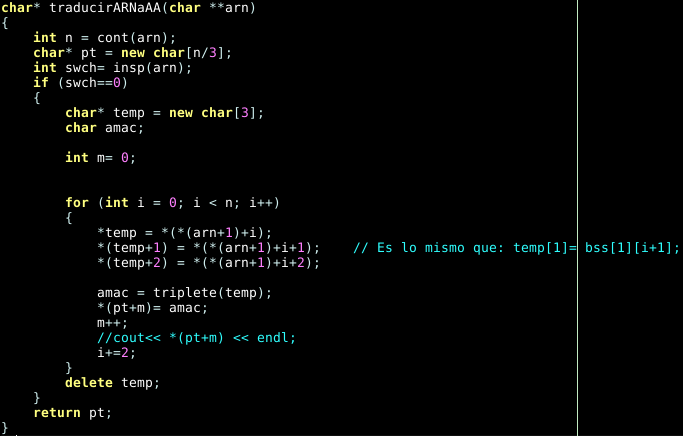
\includegraphics[scale=0.9]{traducir.png}
		\caption{función \texttt{traducirARNaAA}}
		\label{fig:ftrad}
	\end{figure}
	
	\item \texttt{imprimirArregloDeChar}: recibe un puntero de char \texttt{char* a} y un entero \texttt{int n}, e imprime la cantidad especificada de caracteres del puntero.
	
	\begin{figure}[H]
		\centering
		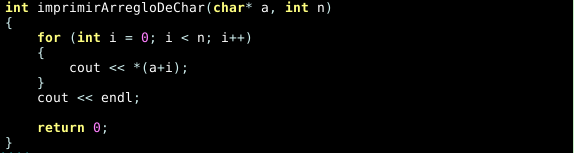
\includegraphics[scale=0.9]{imprimir.png}
		\caption{función \texttt{imprimirArregloDeChar}}
		\label{fig:fimp}
	\end{figure}
	
\end{itemize}
\newpage
\section{Conclusiones}
\begin{itemize}
	\item Cuando no se sabe de antemano la cantidad de elementos con los que el programa va a trabajar se hace uso de la memoria dinámica.
	\item Es responsabilidad del programador liberar el espacio de memoria que se reservó a la hora de crear punteros.
	\item Usando punteros se pueden crear arreglos dinámicos, definiendo el tamaño mientras se ejecuta el programa.	
\end{itemize}
\end{document}
